\chapter{Gradients of all architectures - spectral whitening}\label{appendixD}

\section*{Velocity - Full dataset}\label{sec:velocity-appendixD}

\begin{figure}[!htpb]
\centering
\begin{subfigure}[b]{\textwidth}
   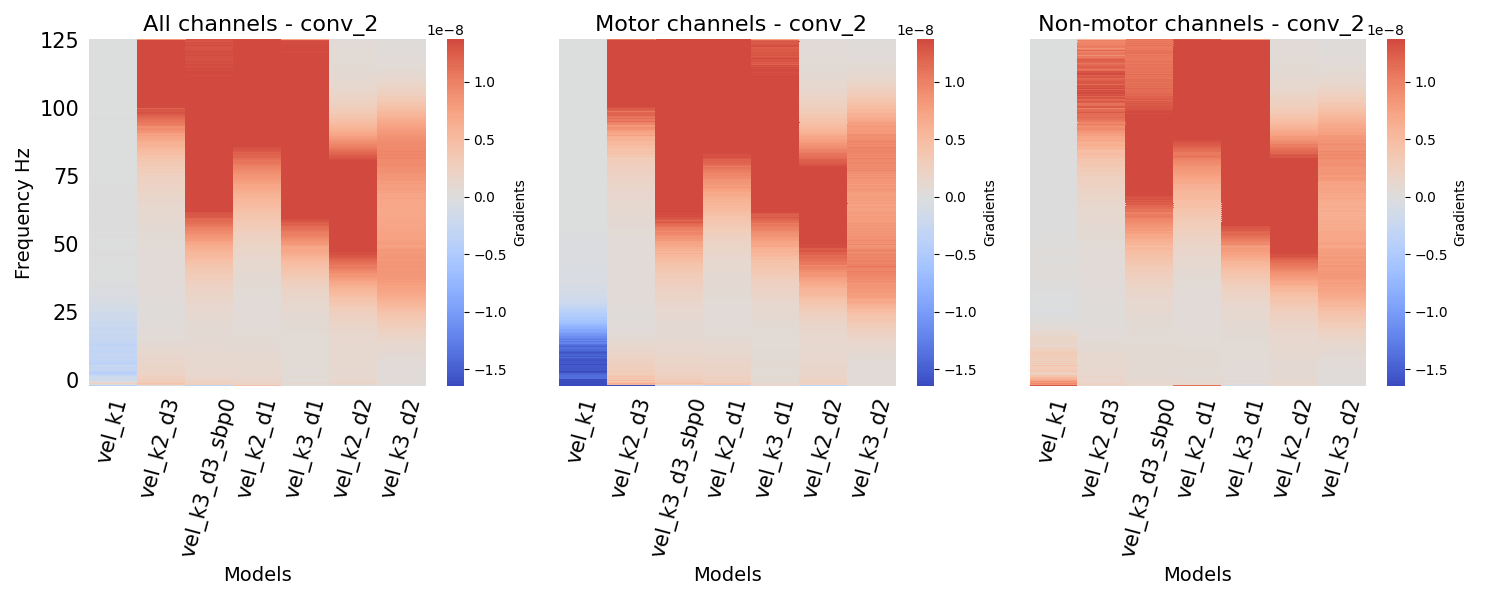
\includegraphics[width=0.85\linewidth]{img/appendix/D/conv-2/m/vel_model_gradients_all_kinds}
   \caption{}
   \label{fig:vel-pw-full-grads-conv-2}
\end{subfigure}

\begin{subfigure}[b]{\textwidth}
   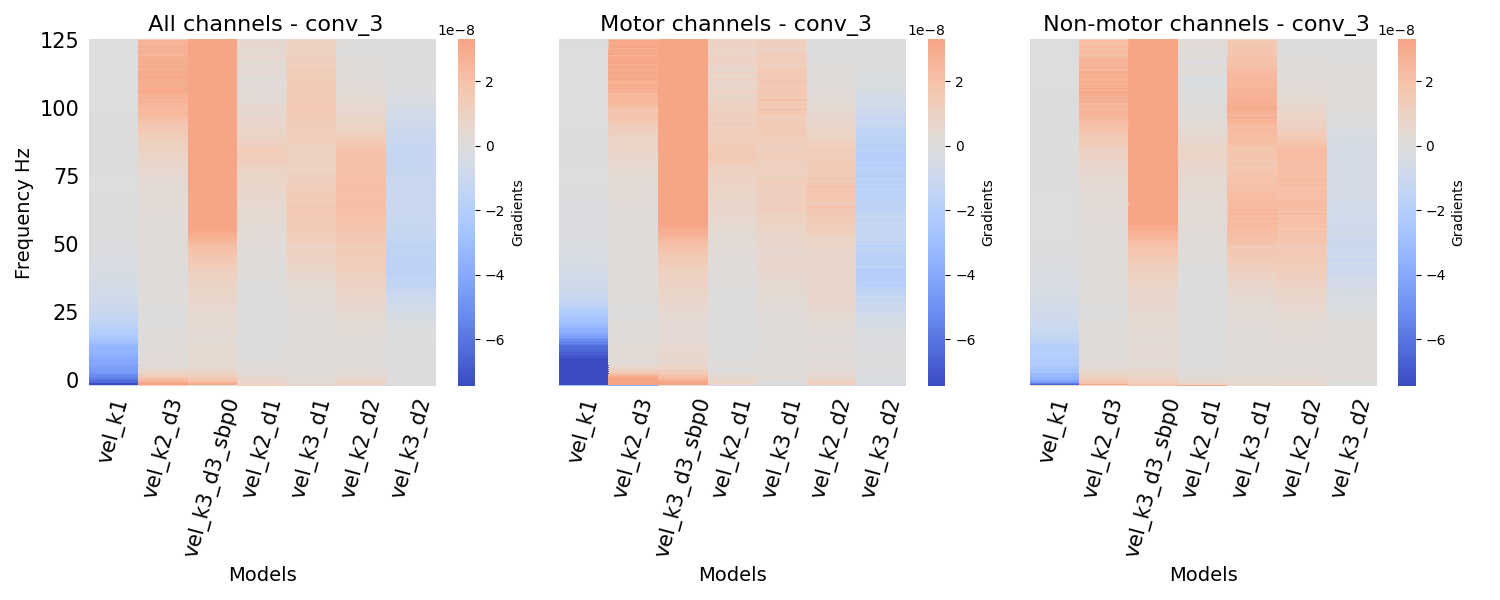
\includegraphics[width=0.85\linewidth]{img/appendix/D/conv-3/m/vel_model_gradients_all_kinds}
   \caption{}
   \label{fig:vel-pw-full-grads-conv-3}
\end{subfigure}
\end{figure}
\clearpage   

\begin{figure}[!htbp]\ContinuedFloat

\begin{subfigure}[b]{\textwidth}
   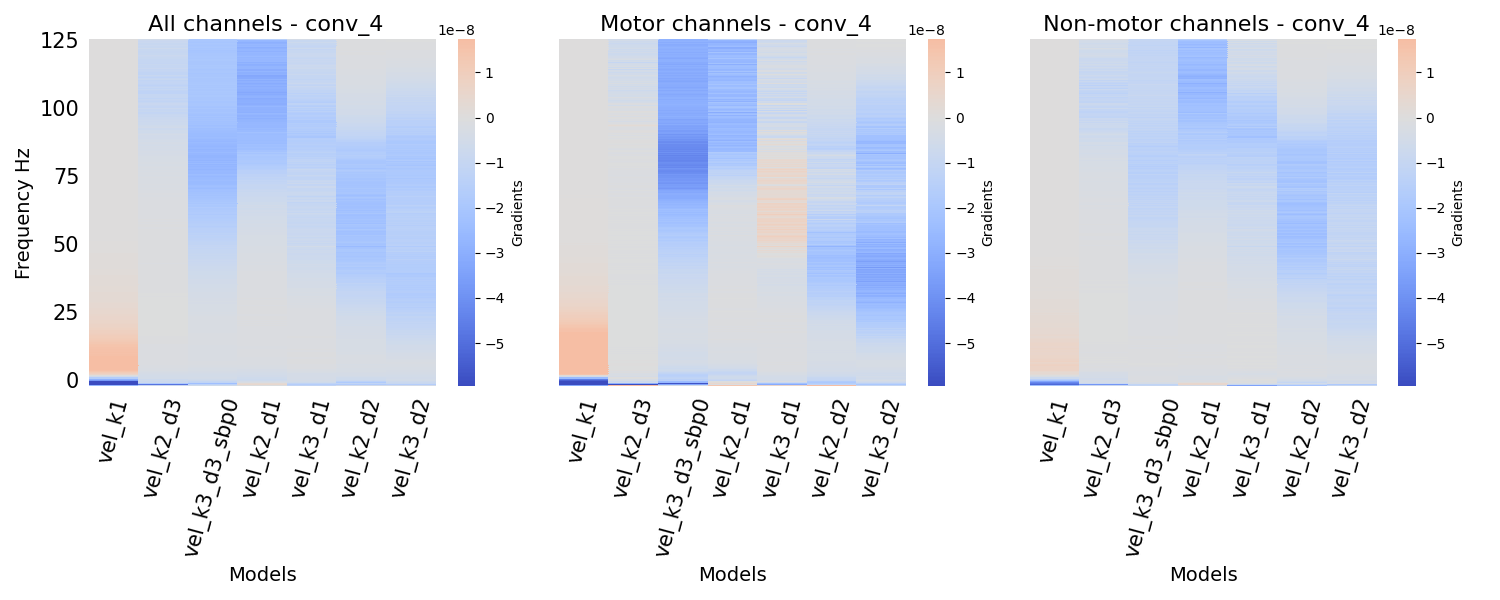
\includegraphics[width=0.85\linewidth]{img/appendix/D/conv-4/m/vel_model_gradients_all_kinds}
   \caption{}
   \label{fig:vel-pw-full-grads-conv-4}
\end{subfigure}

\begin{subfigure}[b]{\textwidth}
   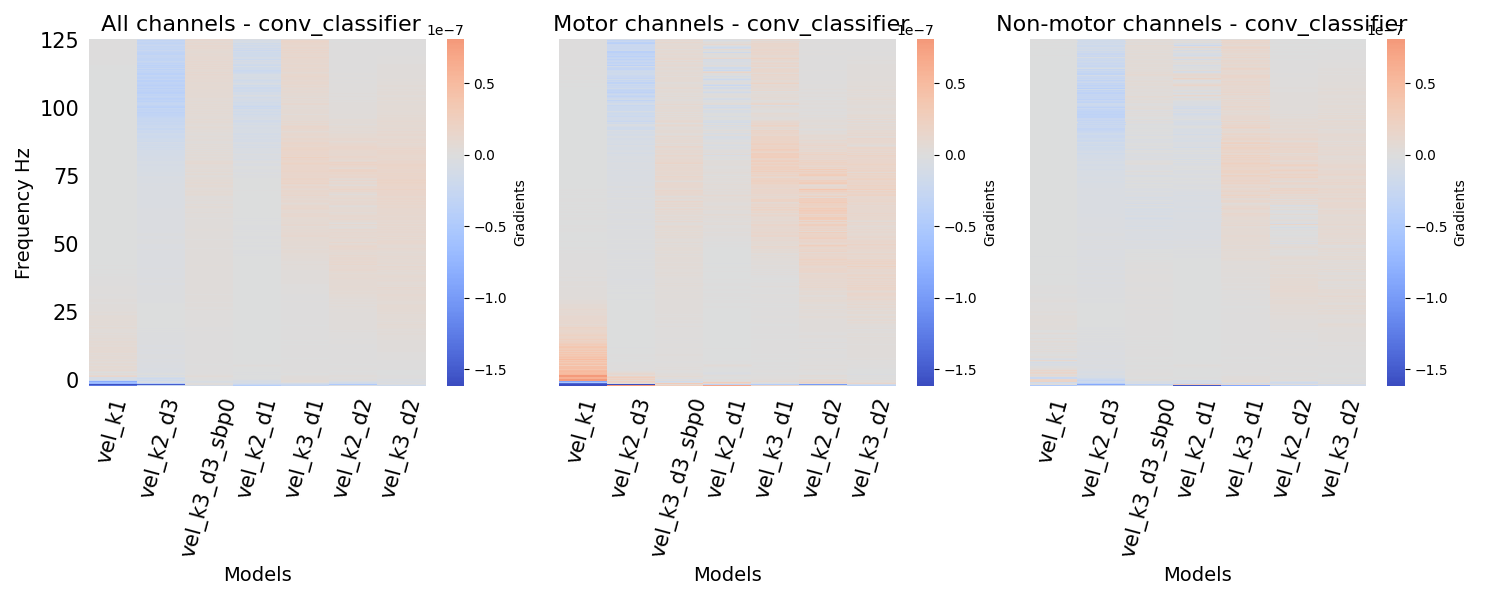
\includegraphics[width=0.85\linewidth]{img/appendix/D/conv-classifier/m/vel_model_gradients_all_kinds}
   \caption{}
   \label{fig:vel-pw-full-grads-conv-classifier}
\end{subfigure}

\caption[]{Gradients of the different CNN architectures decoding velocity from the full whitened dataset in the original non-shifted setting (causal prediction) (see Section~\ref{sec:spectral-whitening}). \textbf{(a)} shows gradients of the convolutional layer in the second block; \textbf{(b)} shows gradients of the convolutional layer in the third block; \textbf{(c)} shows gradients of the fourth convolutional block; \textbf{(d)} shows gradients of the last convolutional layer - the output layer. All channels include channels that do not belong to motor neither non-motor channel sets. See Section \ref{subsec:ieeg-data-preprocessing}}
\label{fig:vel-pw-full-grads}
\end{figure}

\clearpage
\section*{Absolute velocity - High-passed dataset}\label{subsec:vel-high-passed-dataset-appendixD}
\begin{figure}[!htpb]
\centering
\begin{subfigure}[b]{\textwidth}
   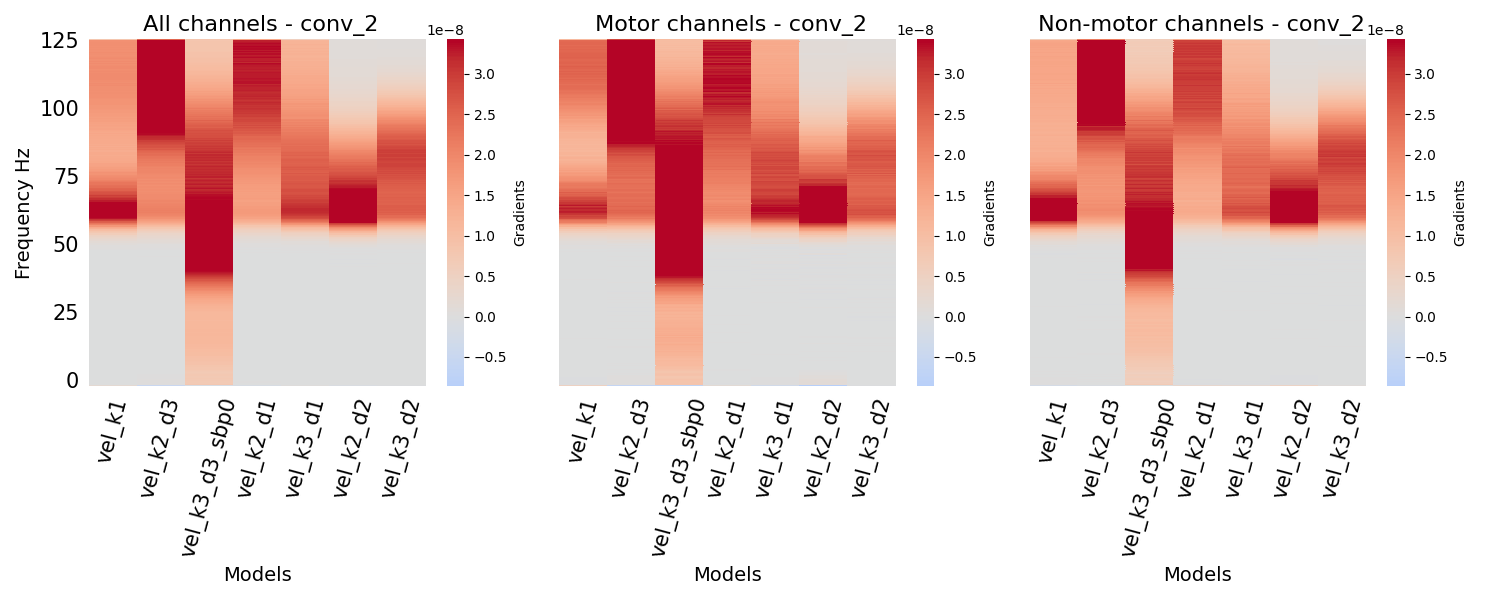
\includegraphics[width=1\linewidth]{img/appendix/D/conv-2/hp-sm/vel_model_gradients_all_kinds}
   \caption{}
   \label{fig:vel-pw-hp-grads-conv-2}
\end{subfigure}

\begin{subfigure}[b]{\textwidth}
   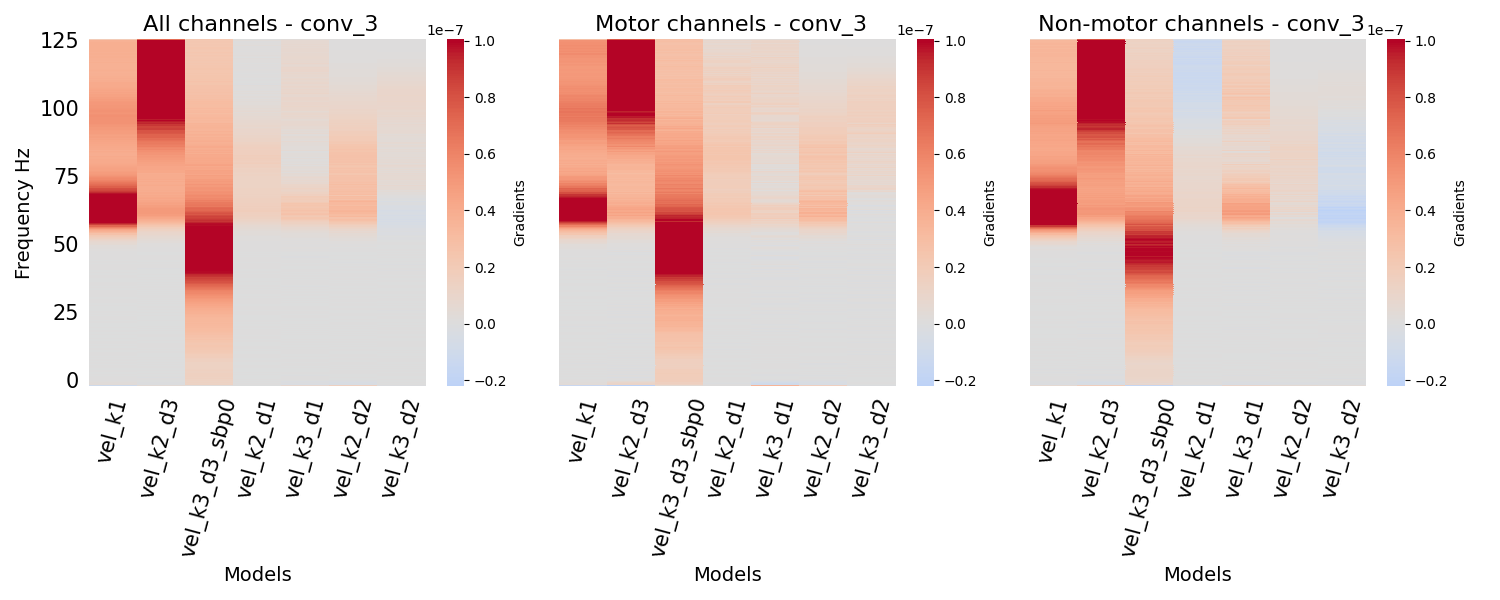
\includegraphics[width=1\linewidth]{img/appendix/D/conv-3/hp-m/vel_model_gradients_all_kinds}
   \caption{}
   \label{fig:vel-pw-hp-grads-conv-3}
\end{subfigure}
\end{figure}
\clearpage   

\begin{figure}[!htbp]\ContinuedFloat

\begin{subfigure}[b]{\textwidth}
   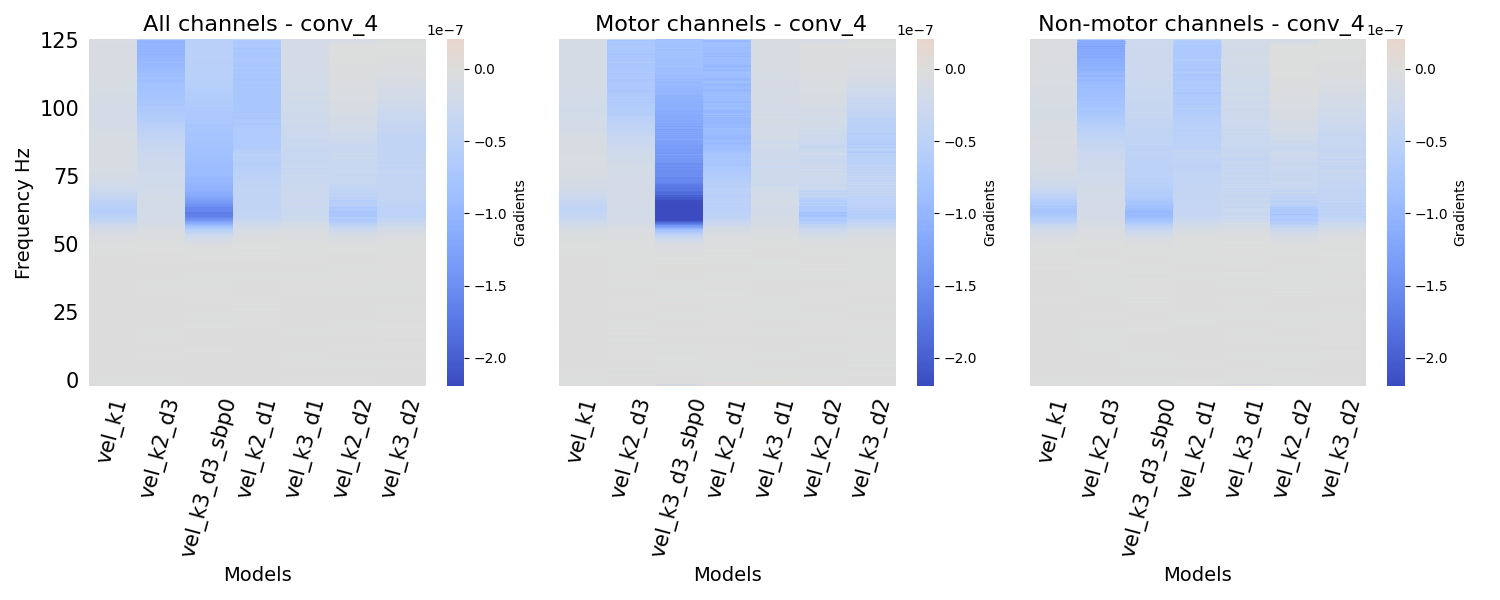
\includegraphics[width=1\linewidth]{img/appendix/D/conv-4/hp-m/vel_model_gradients_all_kinds}
   \caption{}
   \label{fig:vel-pw-hp-grads-conv-4}
\end{subfigure}


\begin{subfigure}[b]{\textwidth}
   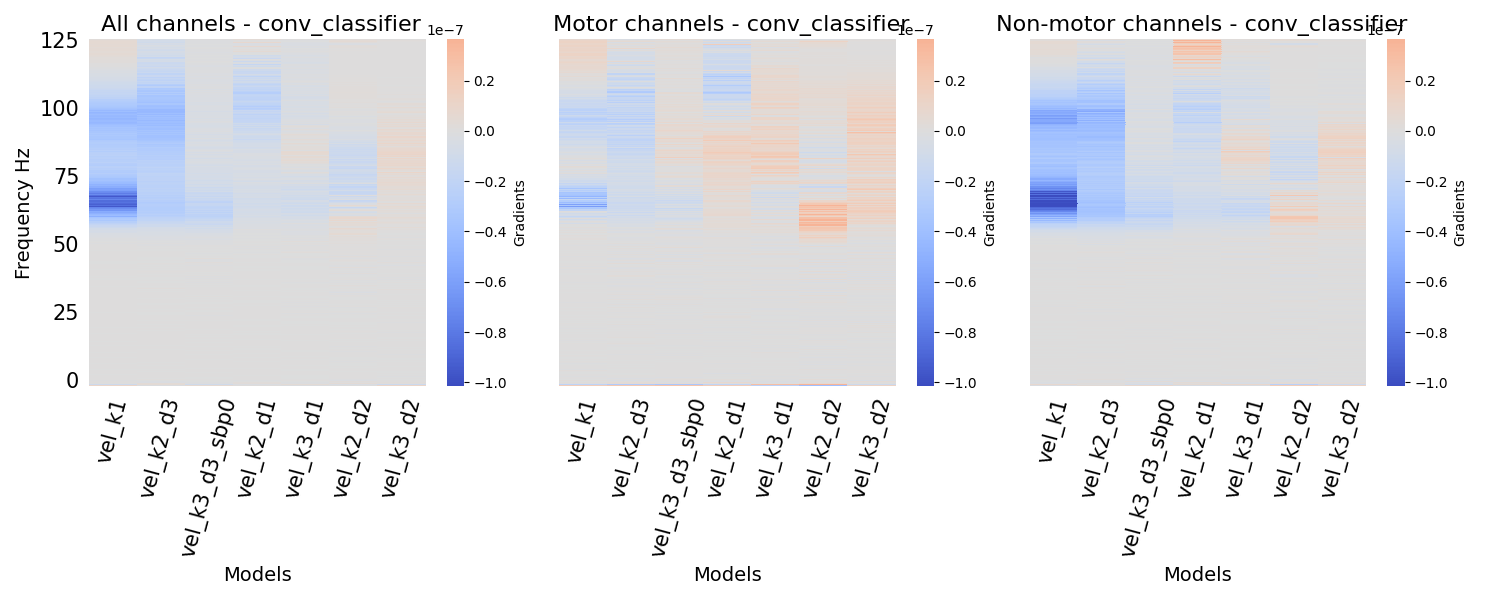
\includegraphics[width=1\linewidth]{img/appendix/D/conv-classifier/hp-m/vel_model_gradients_all_kinds}
   \caption{}
   \label{fig:vel-pw-hp-grads-conv-classifier}
\end{subfigure}

\caption[]{Gradients of the different CNN architectures decoding velocity from the high-passed, whitened dataset in the original non-shifted setting (causal prediction) (see Section~\ref{sec:spectral-whitening}). \textbf{(a)} shows gradients of the convolutional layer in the second block; \textbf{(b)} shows gradients of the convolutional layer in the third block; \textbf{(c)} shows gradients of the fourth convolutional block; \textbf{(d)} shows gradients of the last convolutional layer - the output layer. All channels include channels that do not belong to motor neither non-motor channel sets. See Section \ref{subsec:ieeg-data-preprocessing}}
\label{fig:vel-pw-hp-grads}
\end{figure}

\clearpage
\section*{Absolute velocity - Full dataset}\label{sec:absolute-velocity-appendixD}
\begin{figure}[!htpb]
\centering
\begin{subfigure}[b]{\textwidth}
   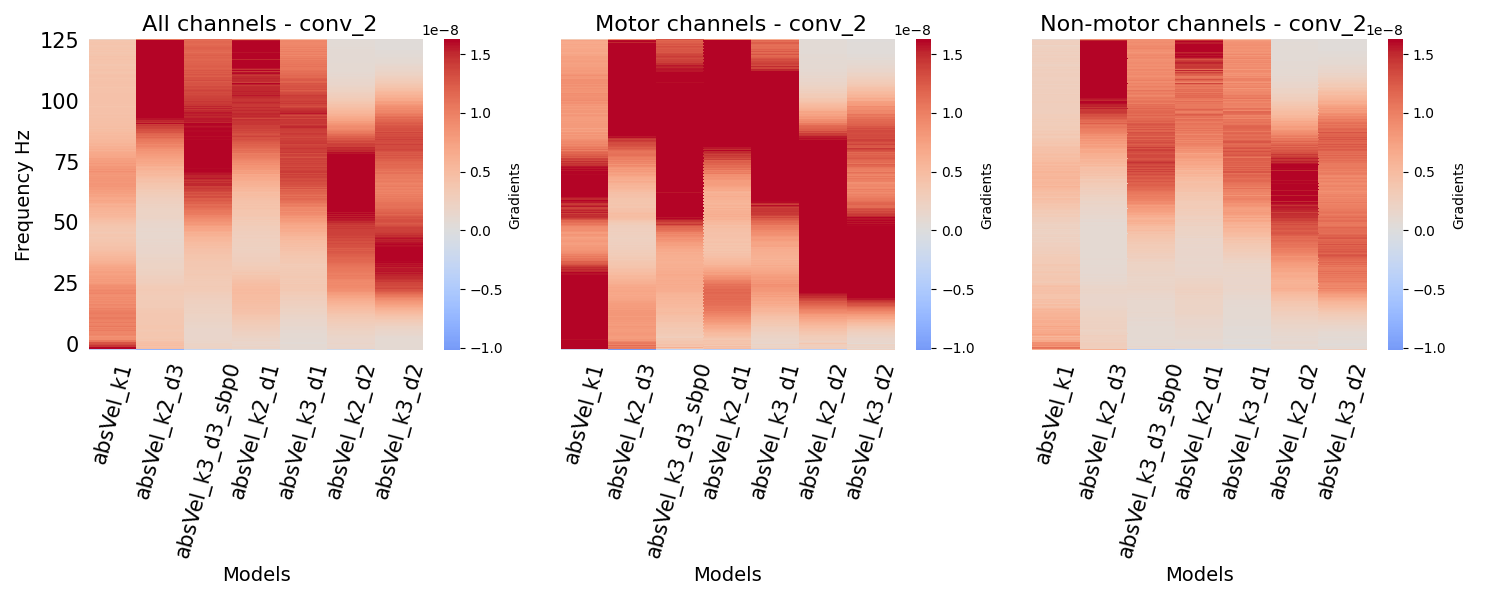
\includegraphics[width=1\linewidth]{img/appendix/D/conv-2/m/absVel_model_gradients_all_kinds}
   \caption{}
   \label{fig:absVel-pw-full-grads-conv-2}
\end{subfigure}

\begin{subfigure}[b]{\textwidth}
   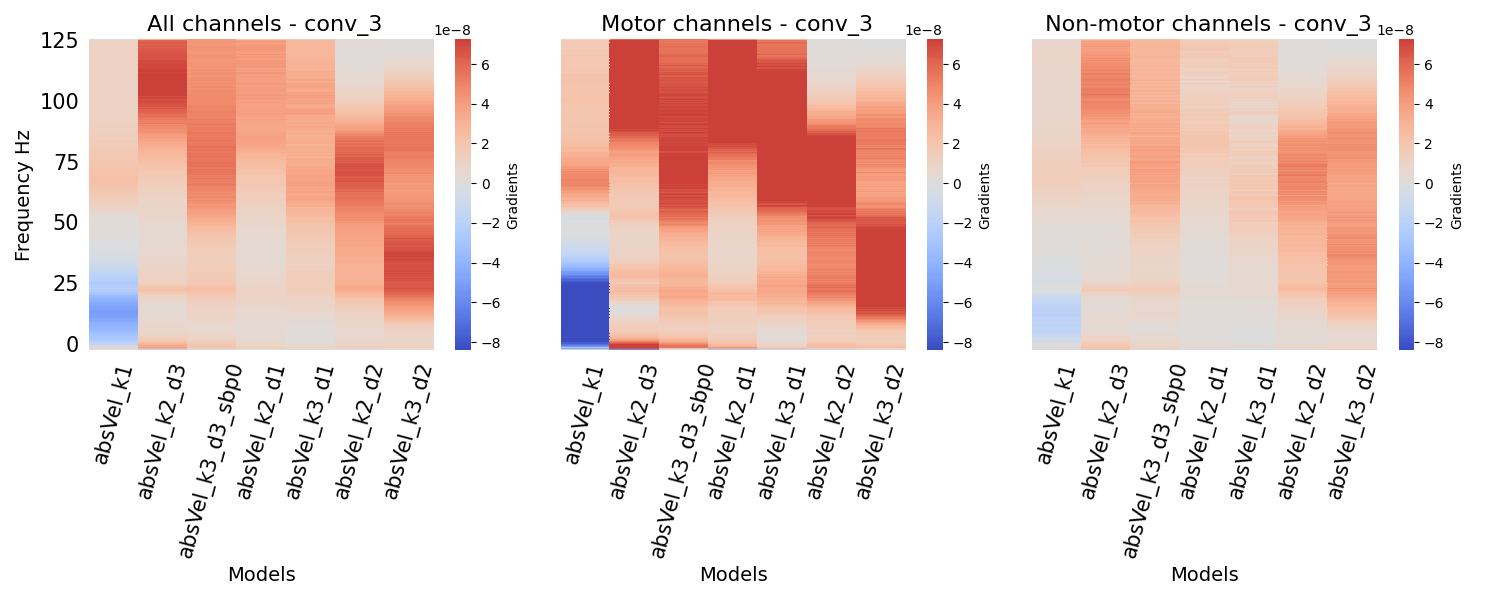
\includegraphics[width=1\linewidth]{img/appendix/D/conv-3/m/absVel_model_gradients_all_kinds}
   \caption{}
   \label{fig:absVel-pw-full-grads-conv-3}
\end{subfigure}
\end{figure}
\clearpage   

\begin{figure}[!htbp]\ContinuedFloat

\begin{subfigure}[b]{\textwidth}
   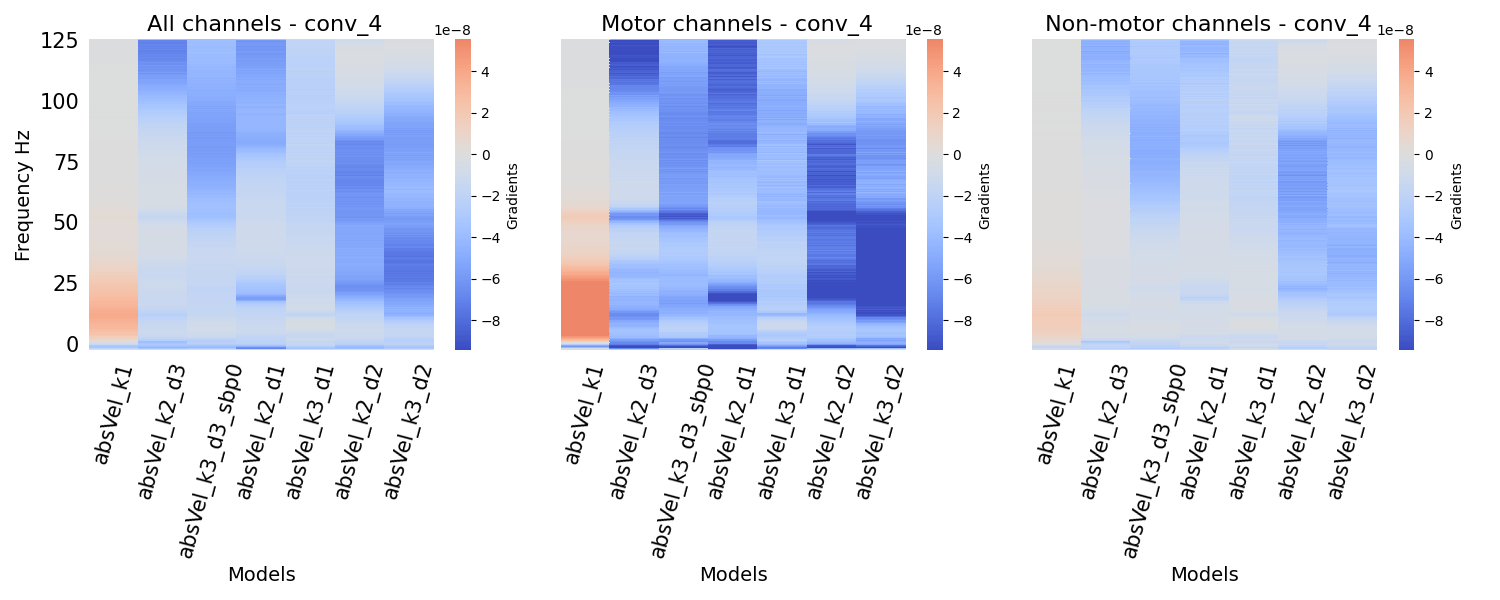
\includegraphics[width=1\linewidth]{img/appendix/D/conv-4/m/absVel_model_gradients_all_kinds}
   \caption{}
   \label{fig:absVel-pw-full-grads-conv-4}
\end{subfigure}

\begin{subfigure}[b]{\textwidth}
   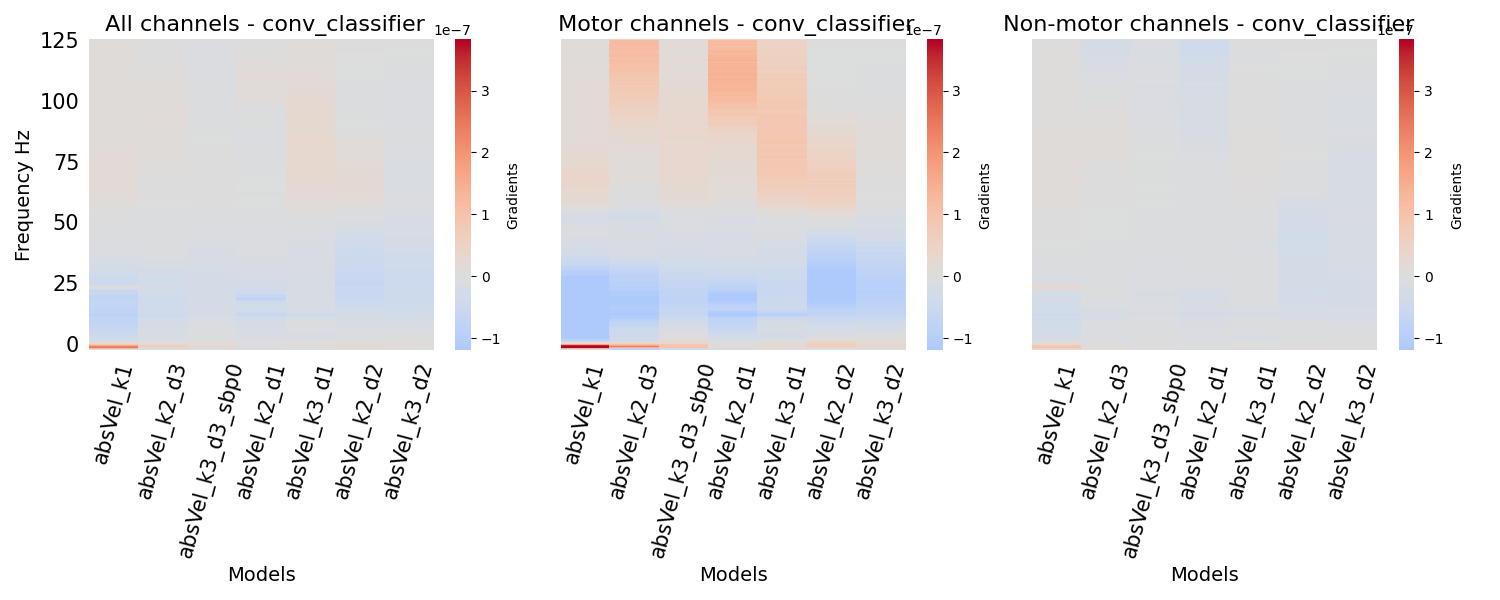
\includegraphics[width=1\linewidth]{img/appendix/D/conv-classifier/m/absVel_model_gradients_all_kinds}
   \caption{}
   \label{fig:absVel-pw-full-grads-conv-classifier}
\end{subfigure}

\caption[]{Gradients of the different CNN architectures decoding absolute velocity from the full whitened dataset in the original non-shifted setting (causal prediction) (see Section~\ref{sec:spectral-whitening}). \textbf{(a)} shows gradients of the convolutional layer in the second block; \textbf{(b)} shows gradients of the convolutional layer in the third block; \textbf{(c)} shows gradients of the fourth convolutional block; \textbf{(d)} shows gradients of the last convolutional layer - the output layer. All channels include channels that do not belong to motor neither non-motor channel sets. See Section \ref{subsec:ieeg-data-preprocessing}}
\label{fig:absVel-pw-full-grads}
\end{figure}

\clearpage
\section*{Absolute velocity - High-passed dataset}\label{subsec:absVel-high-passed-dataset-appendixD}
\begin{figure}[!htpb]
\centering
\begin{subfigure}[b]{\textwidth}
   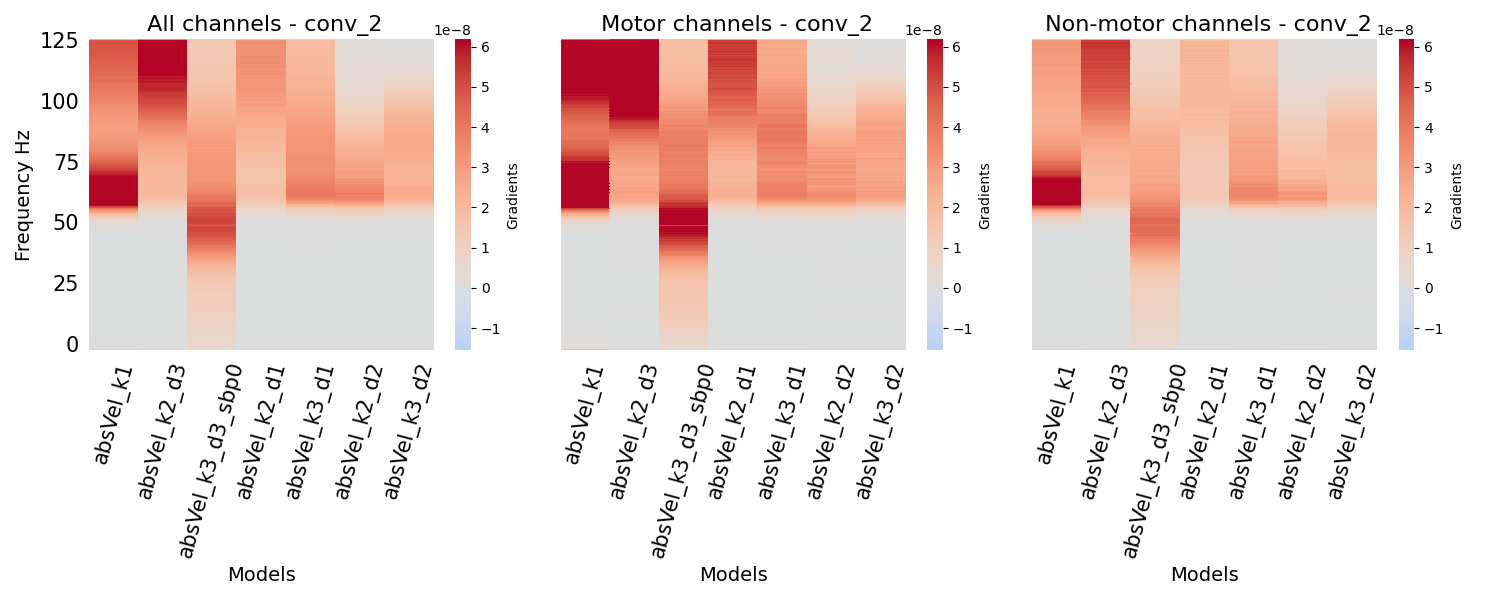
\includegraphics[width=1\linewidth]{img/appendix/D/conv-2/hp-m/absVel_model_gradients_all_kinds}
   \caption{}
   \label{fig:absVel-pw-hp-grads-conv-2}
\end{subfigure}

\begin{subfigure}[b]{\textwidth}
   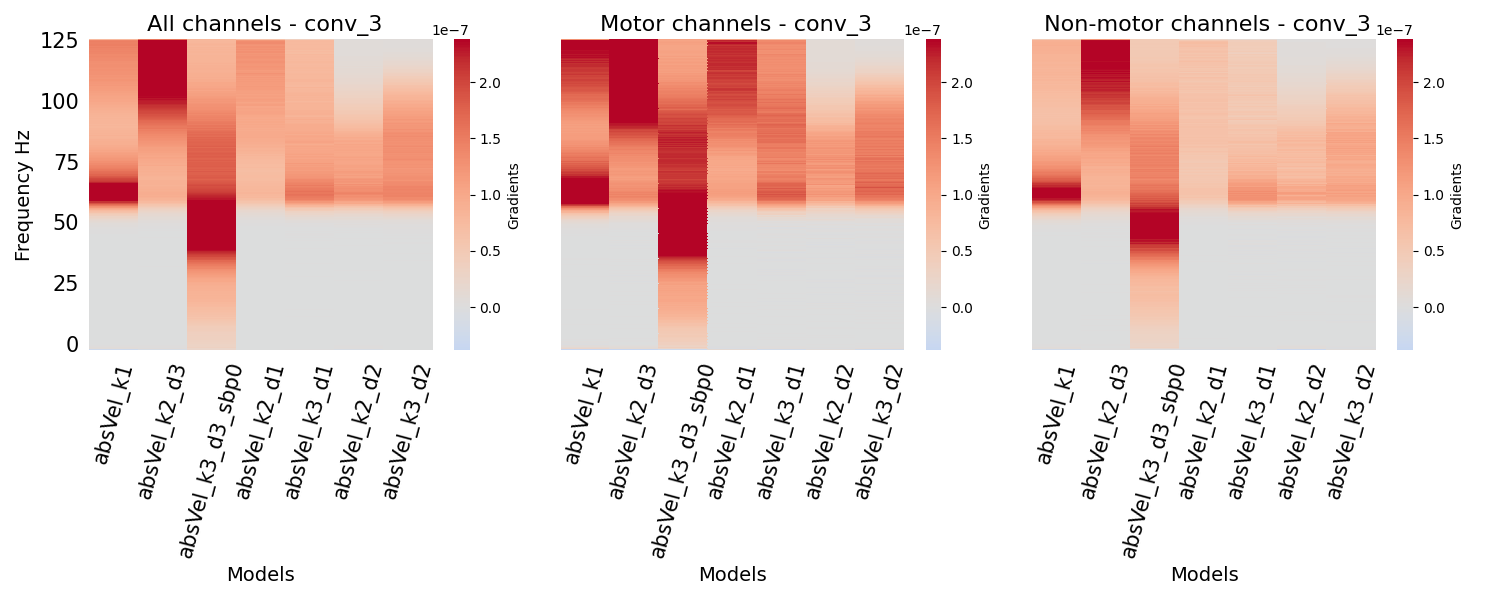
\includegraphics[width=1\linewidth]{img/appendix/D/conv-3/hp-m/absVel_model_gradients_all_kinds}
   \caption{}
   \label{fig:absVel-pw-hp-grads-conv-3}
\end{subfigure}
\end{figure}
\clearpage   

\begin{figure}[!htbp]\ContinuedFloat
\begin{subfigure}[b]{\textwidth}
   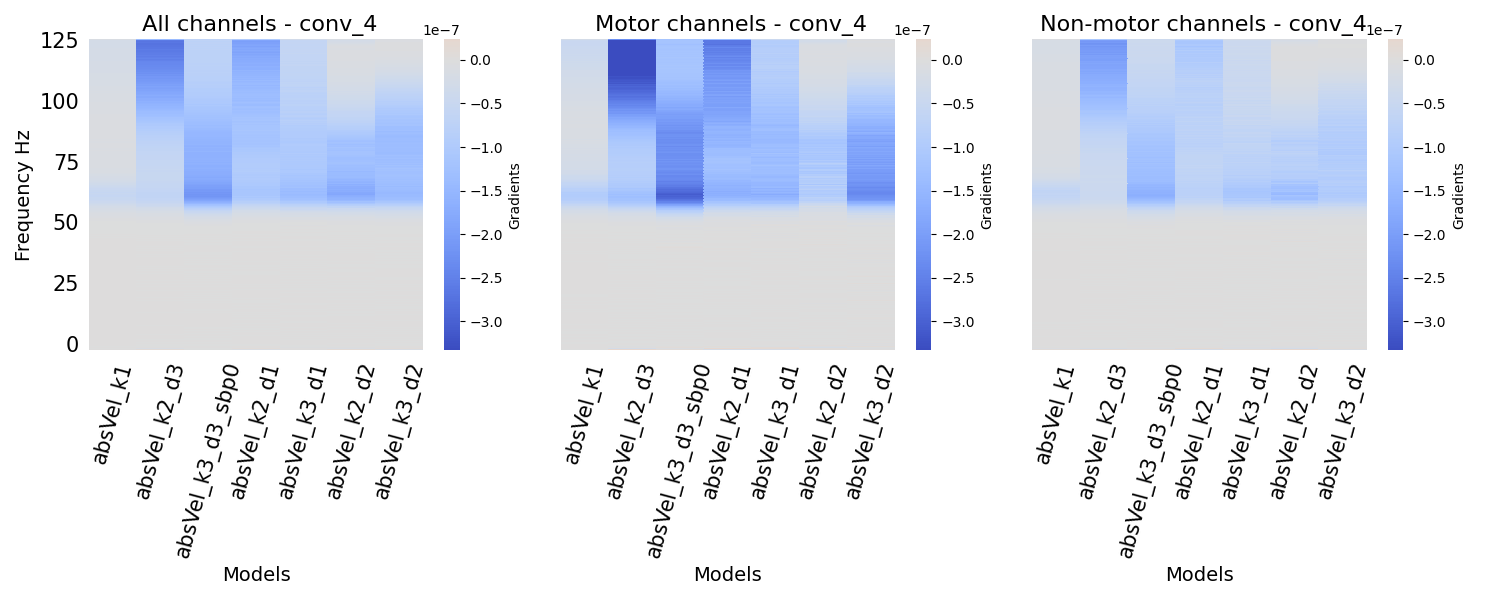
\includegraphics[width=1\linewidth]{img/appendix/D/conv-4/hp-m/absVel_model_gradients_all_kinds}
   \caption{}
   \label{fig:absVel-pw-hp-grads-conv-4}
\end{subfigure}

\begin{subfigure}[b]{\textwidth}
   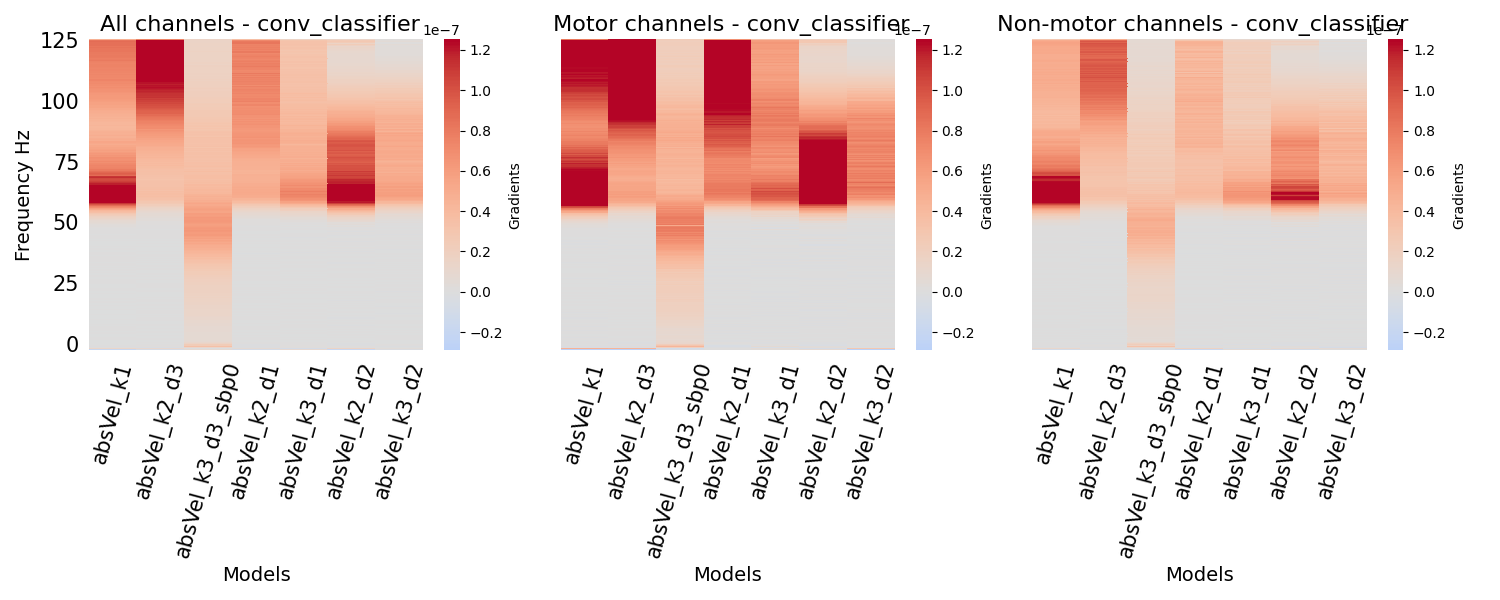
\includegraphics[width=1\linewidth]{img/appendix/D/conv-classifier/hp-m/absVel_model_gradients_all_kinds}
   \caption{}
   \label{fig:absVel-pw-hp-grads-conv-classifier}
\end{subfigure}

\caption[]{Gradients of the different CNN architectures decoding absolute velocity from the high-passed whitened dataset in the original non-shifted setting (causal prediction) (see Section~\ref{sec:spectral-whitening}). \textbf{(a)} shows gradients of the convolutional layer in the second block; \textbf{(b)} shows gradients of the convolutional layer in the third block; \textbf{(c)} shows gradients of the fourth convolutional block; \textbf{(d)} shows gradients of the last convolutional layer - the output layer. All channels include channels that do not belong to motor neither non-motor channel sets. See Section \ref{subsec:ieeg-data-preprocessing}}
\label{fig:absVel-pw-hp-grads}
\end{figure}